\documentclass{article}

\usepackage[english]{babel}
\usepackage[utf8]{inputenc}
\usepackage{amsmath,amssymb}
\usepackage{graphicx}
\usepackage{tikz}
\usetikzlibrary{shapes}
\usepackage{natbib}
\usepackage{hyperref}
\usepackage{listings}

\newcommand{\cmdname}[1]{\texttt{#1}}
\newcommand\footurl[1]{\footnote{\url{#1}}}
\newcommand\urllink[2]{#1\footurl{#2}}
\newcommand\foothref[3]{#1\footnote{\href{#2}{#3}}}
\usepackage{upquote}


\title{Blog}

\author{B1ngster}
\date{}

\begin{document}

\maketitle
\newpage


\tableofcontents
\newpage



\section*{17 May 2023 - \\ Oops! Been down in the dumps, but I rise.}
\addcontentsline{toc}{section}{\protect\numberline{} 17 March 2023 -Oops! Been down in the dumps, but I rise.}

I have not fulfilled my New Year's resolution of making blog posts; there are many reasons I have not found the time. Since my last post, I have been spending time identifying how best to design and put websites into production. An obvious solution is Kubernetes implemented on a cloud host such as Google or Microsoft Azure, but if you run out of credit, your website is going down. There are many other reasons for using a multi-cloud strategy apart from migrating risks; some providers have specific functionality, such as IBM having Watson and Amazon having an easier user interface. 

Indeed, even the best service providers have downtime, which I recently found out as I am currently pointing my domain at my GitHub Page. I have also been using Codespaces. But this may point to a problem with the scalability and availability of Kubernetes when deploying clusters which use code loaded from systems such as GitHub and Docker. Nevertheless, an outage for a version control system is costly to an organisation reducing the team's productivity. As a lone developer, I found this frustrating to use Github to switch between using a laptop and a computer; indeed, Github also has a mobile app. GitLab is popular but only compatible with GitHub if you have a GitLab premium account.

The programming language used in Kubernetes affects the speed of the application. Kubernetes is written in Go; therefore, I have been learning Go, but Rust is a faster programming language... These programming languages are functional programming languages and are highly complex. Most of my previous work has used languages such as PHP, for which I have been receiving many emails asking about my interest in roles. Therefore, I am favouring using Roadrunner, which is a PHP server written in Go, this benefits by enabling the development of websites using the simple syntax of PHP while having the ability to make optimisations using Go.




\section*{5 March 2023 - \\ New Saga: React}
\addcontentsline{toc}{section}{\protect\numberline{}5 March 2023 - New Saga: React}
I have received an email on Indeed asking me to apply for a job as a React developer, and I am applying for it as the job is for a company that delivers a workflow solution for companies in the renewable sector. This aligns with my goals; however, the position requires 4 years of React experience, but I haven't used it in 2 years as it was not used in my dissertation year, and I have not used it while studying MSc Applied Data Science. 

I encountered React several times during my BSc Web Technologies and Digital Media degree as it has features that benefit a developer, especially when features are implemented differently amongst all browsers. I first came across it in my first year; for an assignment, I created a post-it note website; the library simplified creating elements. I also used it due to Redux, which enables state management during an animation assignment.  

I would like to find my old code, but I have probably lost the code in one of my old hard drives or hidden deep in a file system. I find it difficult to look back at old cos because learning new things often helps you identify flaws in the old code. Looking back on the assignments produced, there are many errors to rectify. Unfortunately, this is going to be necessary as I am going to need to find a job.

 \newpage


\section*{1 March 2023 - \\No ID No Online Identity}
\addcontentsline{toc}{section}{\protect\numberline{}1 March 2023 - No ID No Online Identity}

I have purchased a domain off GoDaddy, but I need government-issued identification, which they require to verify your account. Unfortunately, I currently only have a student card, so I will have to wait until the end of the month to get the ID and wait for it. Which may take some time; not only is it expensive, but I also need to get other forms of ID, such as a birth certificate, before I can get that. 

I was looking forward to using GoDaddy because they also have virtual servers, so I could do some programming in languages such as Python and Java; my current provider only has support for PHP. Having a domain would help by not needing to remember IP addresses, and looks more professional. However, there are many other solutions available for now, I am going to use GitHub Pages for hosting, but there is a limit to the number of repositories you can use as Pages; therefore, I have upgraded to GitHub Pro.

\newpage
\section*{28 February 2023 \\ Reflection on Msc Data Science}
\addcontentsline{toc}{section}{\protect\numberline{}28 February 2023 - Reflection on Msc Data Science}


I am reflecting on the last year, 2022 when I was studying Msc Applied Data Science. I thought I had until 4th January; however, in December, I got told this was just a glitch in the system and stopped being a student in September. So the course started on 4th October 2022. I started later that year after receiving my BSc Degree certificate late in October. The course started well, although the first payment I paid to the university for the course didn't go to my account due to my name getting misspelt (thanks to covid masks at the bank). Later, my banks, Eccount and Uaccount, went into administration and buggered up my life.

The course was in the school of engineering, and I learnt a lot that I did not expect:  electrical engineering and renewable energy. In the first semester, we studied Research Methods and Artificial Intelligence for my elective; I did Digital Image and Signal Processing, a 75 percent exam which I was sure I would fail. The others were 50 percent coursework and 50 percent exam. Although I knew I would fail, the subject was interesting...  And if I could figure out where the buttons were on the calculator, I was in for a chance, but I couldn't find the button; I tried to use my newfound knowledge that sine is the derivative of cosine. It didn't work out, but Research Methods have interested me greatly, and that deadline was sooner.
 
In Research Methods. A member of my class and I was teamed with two people from the Msc Renewable Energy course to evaluate monitored data from two real photovoltaic systems located at UCLAN against simulated data. For the assignment, we were assigned roles the people from renewable energy were to provide a literature review, the other person from my course was to do the simulation, and I was the validate the simulated and monitored data. I didn't assign myself the role but took on the part. Our tutor assigned roles; this was strange because the assignment required us to write about using an Agile methodology, and having roles ensured that we used a waterfall methodology. Agile development requires a team to communicate regularly to create an iteration of the product. Unfortunately, the team communicated via WhatsApp, which was unfortunate not having a mobile telephone myself. I thought we were using Microsoft Teams, and everyone was too busy researching.

 \begin{figure}
\caption{Assigned Tasks}
\centering
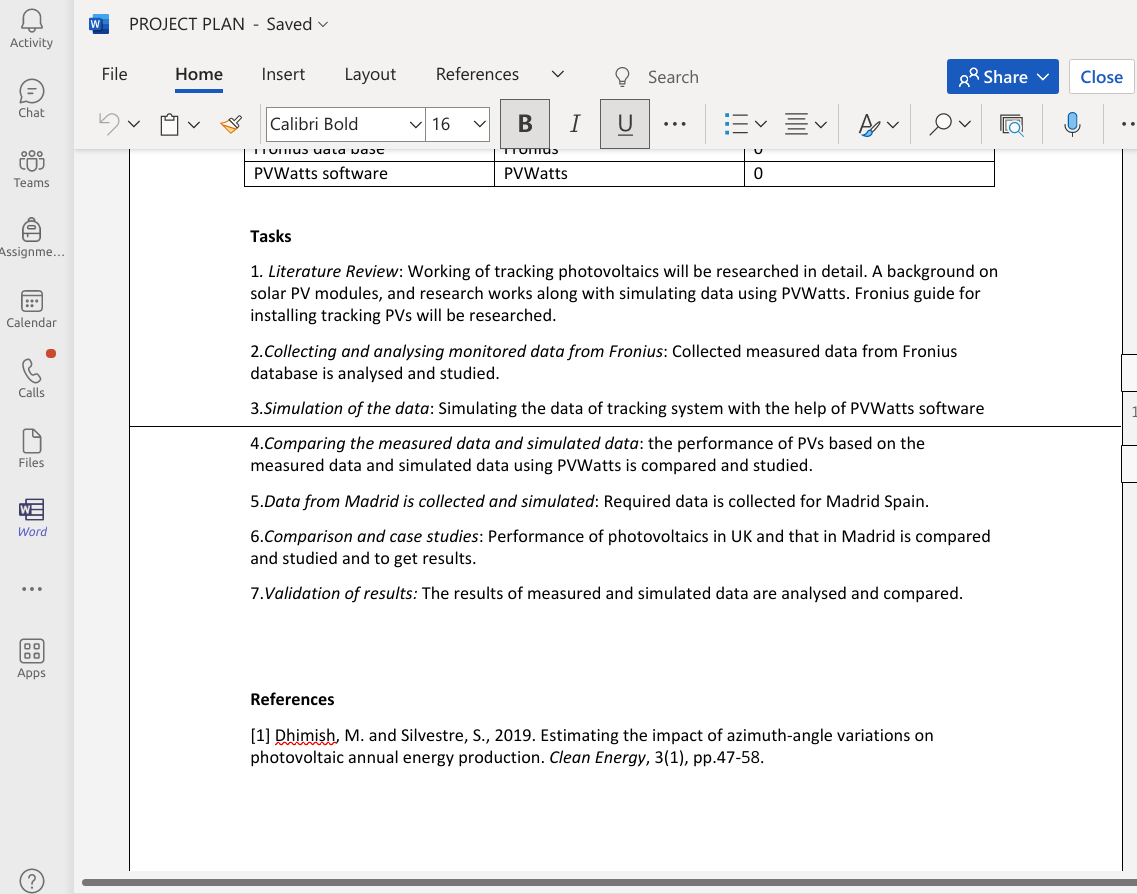
\includegraphics[width=0.5\textwidth]{images/feb/tasklist.png}
\end{figure}
 
\begin{figure}
\caption{The assignment of tasks (not written by myself)}
\centering
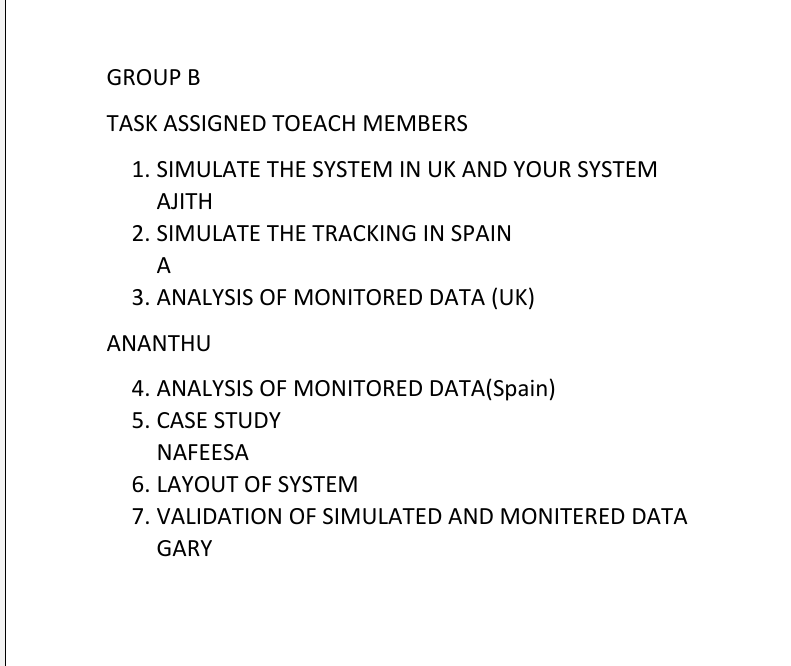
\includegraphics[width=0.5\textwidth]{images/feb/task_list_group.png}
\end{figure}

As you can see, I took on validating the monitored data. So I needed to learn how to verify and validate simulated data. Unfortunately, I did not have experience doing this or a Windows computer to create the simulation (I could have used WINE or a Virtual Machine hired from FFS). So the task was to validate the simulation, ensuring input and output were between a range of possible values. 

There are many ways of modelling a system; it can be modelled in terms of its input and output using equations such as Partial and Ordinary Differential Equations (ODE); they are used to model phenomena such as heat transfer; indeed, photovoltaic systems have similarities with the heat conduction problem as they convert heat into electrical energy. To solve these equations, numerical techniques such as root-finding methods such as the Newton, Secant and polynomial root-finding techniques and often are used when there is no analytical solution. Unfortunately, computer systems are prone to truncation errors due to the finite precision of numbers and are considered unavoidable errors which occur when a continuous function is approximated; another is the effect of solar radiation on the computing system. 

I found the use of polynomials interesting, as this was the first time I had encountered them since school. They were also studied while studying Artificial Intelligence; using them for prediction in regression analysis, the inputs can be modified to measure the effect on output. They provide a simple mathematical model, and the Root Mean Square Error (RMSE) was used to measure improvements made by adding more or fewer polynomials. And solve PDE and ODEs can also be converted into them, although this is what we were still researching at the time. Another interesting thing is that they are used to prove the existence of complex numbers in the Fundamental Theorem of Algebra. And solve PDE and ODE can be converted into equations too - although I was not aware of this then, and the recommended reading pointed to an auto-regressive parameter estimation method.

Bohr's atom model can identify things such as if an atom is likely to be conductive, as it identifies how many and the positions of the electrons in the atom. Neutrons and photons are made of quarks top, bottom, charm, strange, up, and down whereas electrons are fundamental particles like quarks. Bohr's model considers particles to be physical objects orbiting a centre. However, Thomas Young demonstrated the wave–particle duality through the double‐slit experiment in 1802, and the theory is demonstrated in many books on quantum computing; it identifies that electrons do not just act as a particle. Heinrich Hertz proved the existence of electromagnetic waves by using a spark gap transmitter. 

Photocells only use one photon to push the electron into the valence band (or shell), which is the outer shell of electrons and happens photon is within a specific wavelength range. Different materials have different abilities to transmit electricity. This highlights another method - optical modelling, which could determine if the material has deformities, as a photovoltaic cell is made out of different materials, which produce different amounts of electricity. 

Most textbooks create an electrical circuit model; I followed a text recreating it in Matlab, which produced IV curves. Unfortunately, I needed help with the code and requested the book's publisher for its source code, but they only provided that to lectures. I also contacted one of the book's authors, but he didn't have it; the code was from the other author. But by that time, I found other resources. Matlab provides several modelling methods, such as Simulink, where components can be developed in a drag-and-drop interface defining their attributes. I choosen to use the pure code approach, which enabled a greater understanding of the system's inner workings. 

I used Villalva's photovoltaic model, which uses two cells. These account for the non-linearity, but this does not occur just in photovoltaic cells in Duffy (2016) Advanced Engineering highlights the work of Fairweather and Ingham (1941): Subsidence transients in resistors containing none linear resistor with reference to the problem of spark quenching explains that a non-linear component is more realistic in a circuit, having more than a non-linear component has a dramatic effect on the output. Indeed, more than one cell must be simulated as we compare two photovoltaic panels containing many cells. Thankfully, IV curves are also one of the outputs of the PV software. Furthermore, plank's law allows the measurement of energy as discrete values. 

A book provided a model of the sun's irradiation, and a model of the system, if inputs are correct, should give the output that would correspond to that of the real and simulated data. So the data's distribution matched the actual data and the simulated but not the actual values. Indeed the weather also affects the solar array, and forecasting the weather is challenging. Several other things need to be considered: the solar array is connected to an inverter, and the electrical grid to which it is connected imparts their characteristics. The simulation software that was used to recreate the actual data can utilise 3D object files to play locations and the shadows of buildings. Partial shadows and clouds affect the photovoltaic array, which may not have been accounted for. 

Matlab was used for much of the course; it is an appealing language for engineers because it has functions to help solve equations. It requires a licence which prevents it from being portable and expensive, and difficult to scale in Linux: the user needs to run an activation script before startup, which occurs regularly. Fortunately, Octane is open source and uses a similar syntax and features, but it lacks the many plugins Matlab has, such as the Curve Fitting Tool, which we used in Artificial Intelligence. I would like to revisit this code, but I am not enrolled on the course at the time of writing.

In the module: Programming with Data, we used Juypyter Notebooks to program in Python; however, it also supports Julia and R, and the cells can be annotated with Markdown and render Latex. During Artificial Intelligence, we used Juypyter Notebooks, Python and TensorFlow during a class about Deep Learning. I noted the difficulty I was having with producing equations in Microsoft Word, finding using writing them in Latex a better alternative to the drag-and-drop interface which it offered. Indeed, in the second coursework of Programming with Data, we used  R, which too supports Latex via R Markdown. The good thing about being able to use equations in your code is to be able to share code with people who are not familiar with the programming language and to use proofs and reasoning; a cool thing I would like to see is a library to compile equations into computer programs, and I don't think it is far too from been developed.

\newpage

 \end{document}
